% !TeX program = pdflatex
\documentclass[conference,letterpaper]{IEEEtran}
\usepackage{amsmath,amssymb,graphicx,booktabs,array,listings,url,microtype}
\usepackage{placeins}
\usepackage[hidelinks]{hyperref}
\graphicspath{{figures/}}
\newcommand{\code}[1]{\nolinkurl{#1}}
\newcolumntype{L}[1]{>{\raggedright\arraybackslash}p{#1}}
\lstset{language=Python,basicstyle=\ttfamily\scriptsize,breaklines=true,columns=fullflexible,keepspaces=true,showstringspaces=false,frame=single,tabsize=4}
\hypersetup{pdftitle={Camera Motion from ArUco Markers: ME 566 Homework 4},pdfauthor={Jordan Brown}}
\newcommand{\Endpoint}{80.341}
\newcommand{\EndpointError}{4.141}
\newcommand{\CumulativeRMSE}{3.318}
\newcommand{\SigmaPixel}{0.577}
\newcommand{\EndpointCI}{0.330}
\newcommand{\SharedRxSD}{0.386}
\newcommand{\SharedRySD}{0.095}
\newcommand{\SharedRzSD}{0.735}
\title{Camera Motion from ArUco Markers}
\author{\IEEEauthorblockN{Jordan Brown}\IEEEauthorblockA{ME 566\\Homework 4: Camera Motion}}
\begin{document}
\maketitle
\noindent\textbf{AI Use Disclosure:} AI assistance (OpenAI Codex) was used for code development, numerical analysis, and writing and formatting this report.
\par\medskip
\begin{abstract}
A calibrated camera observes a stationary 10 cm ArUco marker during a translation sequence. Eleven photographs at 3-inch (7.62 cm) intervals span an expected 76.2 cm, exceeding the required 30 cm. The program detects the marker, draws its outline and coordinate axes, and fits one shared orientation with a separate translation for each image, matching the reported fixed-orientation acquisition. The estimated endpoint displacement is 80.34 cm, with a mean interval of 8.06 cm and interval RMSE of 0.86 cm. A Jacobian-based calculation estimates pose uncertainty conditional on fixed calibration, exact marker size, and zero camera rotation. Full equations, coordinate conventions, function parameters, measured results, and reproduction commands accompany the source code.
\end{abstract}
\begin{IEEEkeywords}ArUco, camera calibration, pose estimation, translation, uncertainty\end{IEEEkeywords}

\section{Task 1: Marker Detection and Coordinate Frames}
\subsection{Printed marker and observations}
The stationary marker is attached to a flat wall. Its outer black square measures $L=0.10$ m on each side; white paper margins are excluded. It decodes as ID 0 in \code{DICT_4X4_50}, a dictionary of 50 markers with $4\times4$ internal binary cells. The 11 JPEG photographs are $2992\times2992$ pixels and are processed in timestamp filename order. Camera metadata identifies a Samsung Galaxy S23 FE; a first-image spot check in both the calibration and marker sets records 5.54 mm focal length, 23 mm equivalent, and digital zoom 1.0. Capture settings are not independently verified for every image.

For a repeat print, generate ID 0 using the code below, print without aspect-ratio distortion, and measure the black square with a ruler. Adjust print scaling until its side is 10 cm; pixel count alone does not set physical print size. Attach it flat and keep it stationary throughout acquisition.
\begin{lstlisting}
dictionary = cv2.aruco.getPredefinedDictionary(
    cv2.aruco.DICT_4X4_50)
marker = cv2.aruco.generateImageMarker(
    dictionary, 0, 600, borderBits=1)
cv2.imwrite('marker_id0.png', marker)
\end{lstlisting}
The detector uses subpixel corner refinement, returns clockwise corner order beginning at the decoded top-left, and draws the quadrilateral and ID with \code{drawDetectedMarkers}. OpenCV's ArUco tutorial documents these operations~\cite{aruco}. A valid pose requires all projected object corners to lie in front of the camera and independent initialization reprojection RMSE no greater than 3 pixels. ID 0 is detected and accepted in all 11 observations.

\begin{figure*}[t]\centering
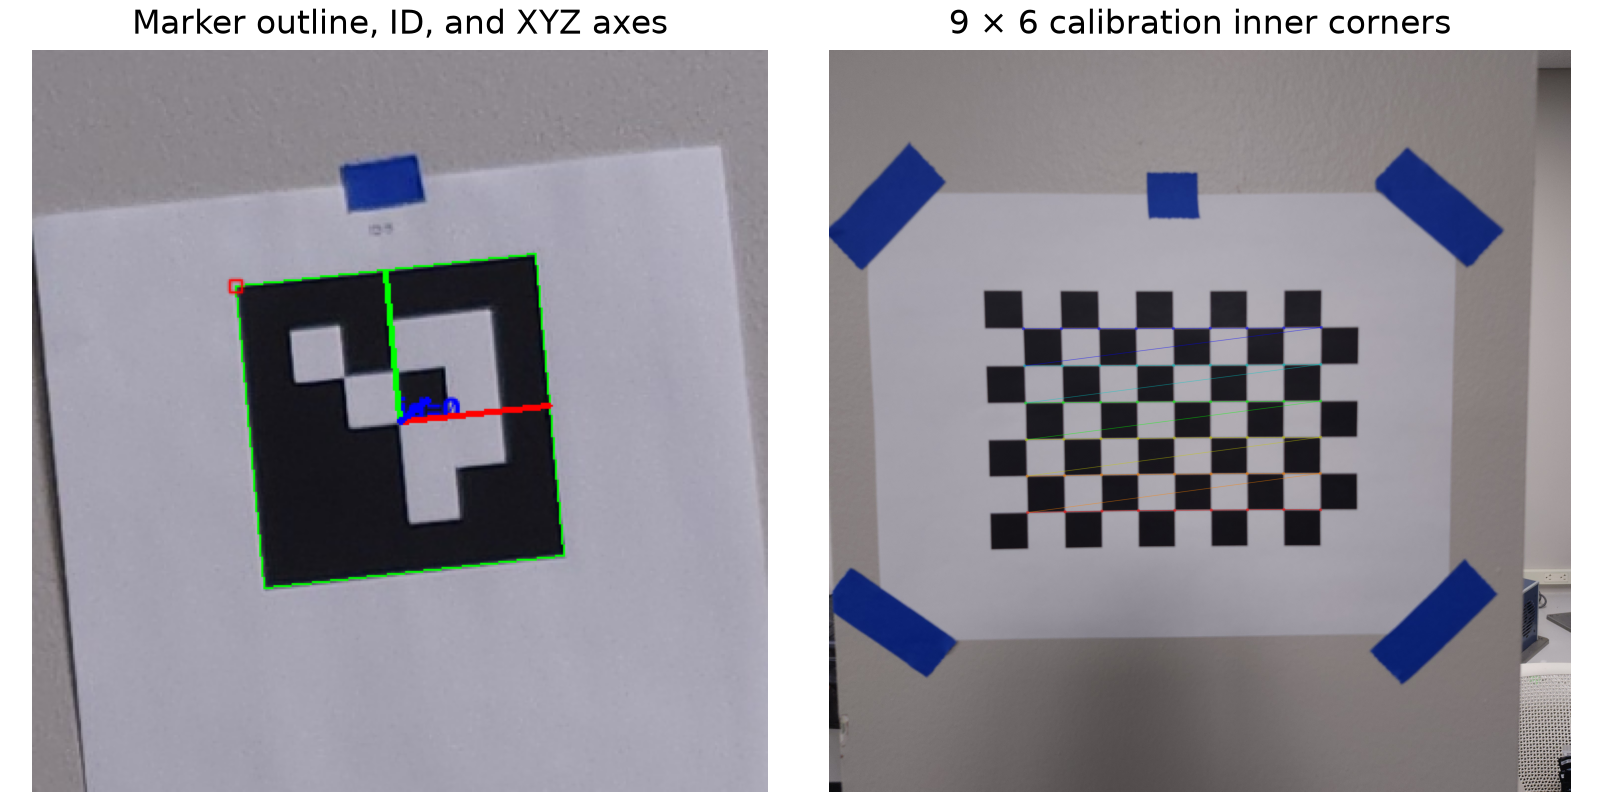
\includegraphics[width=.78\textwidth]{marker_and_calibration.png}
\caption{Left: close view of the detected marker, labeled outline, and centered coordinate frame. The frame axes are X red, Y green, and Z blue. Right: detected $9\times6$ inner-corner calibration grid. Images are resized only for report display; estimation uses full resolution.}\label{fig:marker}
\end{figure*}

\subsection{Coordinate definitions}
The marker frame $M$ has its origin at the black square's center, X to the printed right, Y upward, and Z outward from the printed face. Ordered 3D corners, in meters, are
\begin{equation}
\begin{aligned}
P_1&=(-L/2,L/2,0),&P_2&=(L/2,L/2,0),\\
P_3&=(L/2,-L/2,0),&P_4&=(-L/2,-L/2,0).
\end{aligned}
\end{equation}
Each camera frame $C_i$ uses X right, Y down, and Z forward. A rigid transform
\begin{equation}
T_{C_i\leftarrow M}=\begin{bmatrix}R_i&t_i\\0&1\end{bmatrix},\quad
p_{C_i}=R_iP_M+t_i
\end{equation}
therefore maps marker points into camera coordinates. $R_i$ is a $3\times3$ rotation and $t_i$ is a three-component translation in meters. \code{drawFrameAxes} draws this marker frame using axis length $0.05$ m and line thickness 2 pixels. Figure~\ref{fig:sequence} shows full annotated frames.

\section{Task 2: Measurable Camera Translation}
The acquisition measurements supplied for this sequence specify successive camera positions separated by 3 inches, with no camera rotation. Since $1$ inch is $0.0254$ m, the expected interval is
\begin{equation}d_{\mathrm{ref}}=3(0.0254)=0.0762\ \mathrm{m}.
\end{equation}
Frame $i$ is compared with nominal initial-frame displacement $i d_{\mathrm{ref}}$, for $i=0,\ldots,10$. This comparison assumes the reported steps follow the same translation direction. It does not independently measure the displacement direction.

To repeat the measurable acquisition, mark 11 positions on a straight guide at 7.62 cm spacing using a ruler or tape. Align the same reference point on the camera support with each position, keep the camera rigidly oriented, and take one image after it settles. Keep the same lens, image crop, resolution, and focus for calibration and marker capture. The existing captures establish the supplied spacing and orientation description; the particular translation support and ruler tolerance were not recorded, so this report does not assign them an invented accuracy. The reference spacing is used only for evaluating the final estimates, never as a constraint in the image fit.

\section{Task 3: Motion Relative to the Initial Frame}
\subsection{Camera calibration}
The calibration set contains 59 checkerboard photographs at the marker-image resolution. A $9\times6$ inner-corner grid is detected in 48 views. Those 48 views enter \code{calibrateCamera}; the other 11 do not provide a detected grid. Object points are $(a,b,0)$ for integer column $a=0,\ldots,8$ and row $b=0,\ldots,5$. Unit square spacing is sufficient because only intrinsics and distortion are used; checkerboard translations are not used to set ArUco motion scale. Calibration RMS is 0.819 pixels.

The fitted intrinsic matrix in pixels is
\begin{equation}
K=\begin{bmatrix}
2816.1017&0&1524.3629\\
0&2803.5592&1459.6101\\0&0&1
\end{bmatrix}.
\end{equation}
The coefficient vector $(k_1,k_2,p_1,p_2,k_3)$ is approximately $(0.212416,-0.284289,-0.002481,-0.003162,-2.411326)$. JSON preserves full precision. For a camera-coordinate point $(X,Y,Z)$, define $x=X/Z$, $y=Y/Z$, and $\rho^2=x^2+y^2$. Projection with the five-coefficient distortion model~\cite{calib} is
\begin{align}
A&=1+k_1\rho^2+k_2\rho^4+k_3\rho^6,\\
x_d&=xA+2p_1xy+p_2(\rho^2+2x^2),\\
y_d&=yA+p_1(\rho^2+2y^2)+2p_2xy,\\
u&=f_xx_d+c_x,\qquad v=f_yy_d+c_y.
\end{align}
Here $f_x,f_y$ are pixel focal lengths and $c_x,c_y$ are principal-point coordinates. Call the resulting mapping $\pi(K,d,RP+t)$. Raw distorted images are supplied to pose estimation with $K,d$; images are not undistorted a second time. The mathematical scale of marker translation comes from the measured $L$, not from calibration-board units.

\subsection{Shared-orientation pose fit}
For this fixed-orientation experiment, $R_i=R$ across all images. Given observed corners $q_{ij}\in\mathbb R^2$, the final parameters minimize
\begin{equation}
\widehat\theta=\arg\min_{r,t_0,\ldots,t_{10}}
\sum_{i=0}^{10}\sum_{j=1}^{4}
\|\pi(K,d,R(r)P_j+t_i)-q_{ij}\|^2.
\label{eq:fit}
\end{equation}
$r$ is a three-component Rodrigues rotation vector, converted to $R$ by \code{Rodrigues}. There are 36 parameters: three shared rotation components and 33 translation components. Calibration and marker size remain fixed. There is no constant-step, constant-speed, straight-path, or known-spacing term in this objective. It enforces fixed orientation but leaves all translations free.

Independent iterative PnP solutions initialize each $t_i$. Each initialized rotation is tried as a shared starting rotation. SciPy \code{least_squares} performs Levenberg--Marquardt optimization of the pixel residuals, with \code{method='lm'}, \code{max_nfev=3000}, and \code{ftol=xtol=gtol=1e-11}. These tolerances control termination based on objective change, parameter change, and gradient criteria; the evaluation budget bounds optimization. The converged positive-depth candidate with lowest squared pixel residual is selected. This is a batch fit using all images, not an online estimate.

\subsection{Initial-camera-relative motion}
The general initial-relative camera transform is
\begin{equation}
T_{C_0\leftarrow C_i}=T_{C_0\leftarrow M}
(T_{C_i\leftarrow M})^{-1}.
\end{equation}
With common rotation,
\begin{equation}
T_{C_0\leftarrow C_i}
=\begin{bmatrix}RR^T&t_0-RR^Tt_i\\0&1\end{bmatrix}
=\begin{bmatrix}I&t_0-t_i\\0&1\end{bmatrix}.
\label{eq:relative}
\end{equation}
Thus the camera position is $p_i=t_0-t_i$ expressed in the initial camera's axes; $p_0=0$. Relative rotation is identity by the capture constraint, not a separately verified result. Each displacement is referenced directly to frame 0, rather than accumulated from estimated intervals. Initial displacement magnitude and consecutive step length are
\begin{equation}
D_i=\|p_i\|_2,\qquad s_i=\|p_i-p_{i-1}\|_2\quad(i>0).
\end{equation}

\section{Task 4: Agreement with Measurable Motion}
Ten 7.62 cm intervals span 76.2 cm, comfortably exceeding the 30 cm requirement. The final initial-relative displacement is $\Endpoint$ cm. Its signed endpoint difference is $+\EndpointError$ cm, approximately 5.4\% of the expected span. Average estimated step is 8.059 cm, compared with 7.620 cm expected, a signed mean difference of 0.439 cm (5.8\%).

For $N=11$ observations, the two comparison errors are
\begin{align}
E_{\mathrm{step}}&=\sqrt{\frac1{N-1}\sum_{i=1}^{N-1}(s_i-d_{\mathrm{ref}})^2},\\
E_{\mathrm{initial}}&=\sqrt{\frac1N\sum_{i=0}^{N-1}(D_i-i d_{\mathrm{ref}})^2}.
\end{align}
They equal 0.861 cm and $\CumulativeRMSE$ cm, respectively. The last step is 5.897 cm; the full set is retained. The mean does not imply every interval is equally accurate. Joint marker reprojection RMS is 0.627 pixels, measuring image-fit consistency rather than external measurement accuracy.

\begin{figure*}[t]\centering
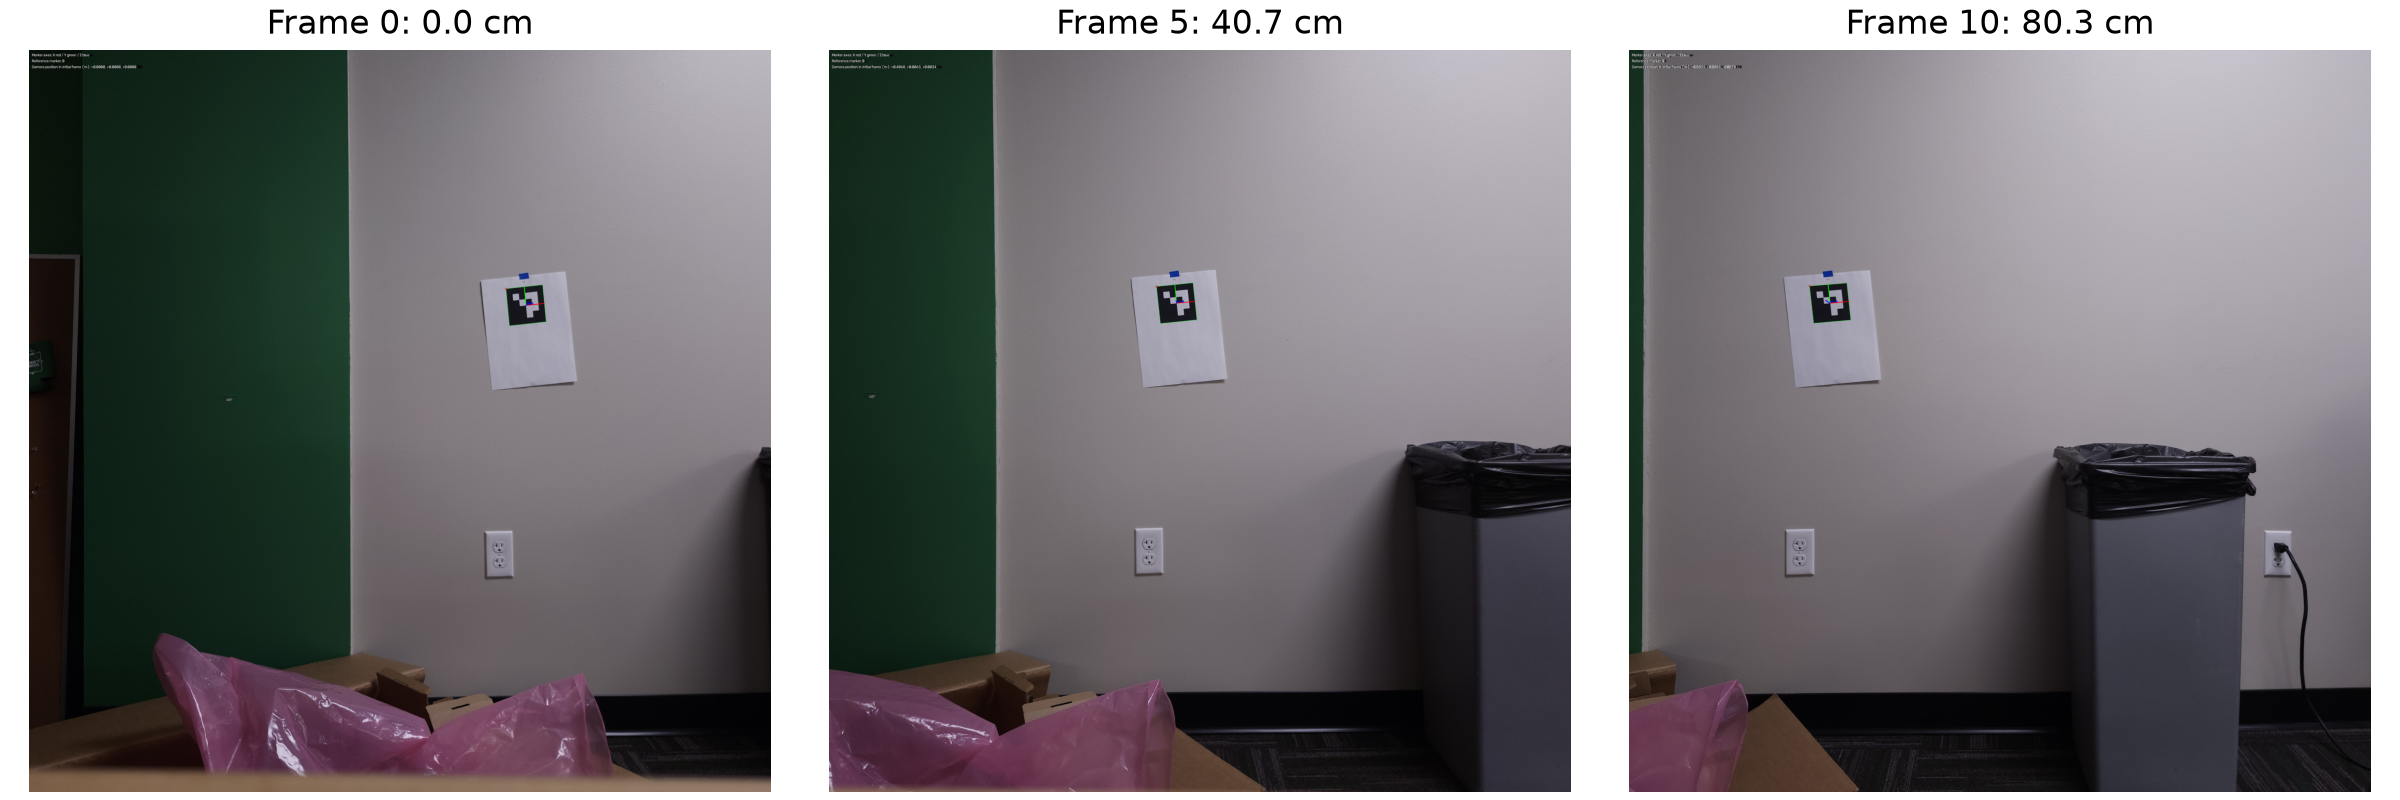
\includegraphics[width=\textwidth]{annotated_sequence.png}
\caption{Frames 0, 5, and 10 from the 11-image sequence. Each output includes the marker outline, ID, and coordinate axes. Positions refer to the initial camera frame, while the drawn axes are the marker frame.}\label{fig:sequence}
\end{figure*}
\begin{figure}[t]\centering
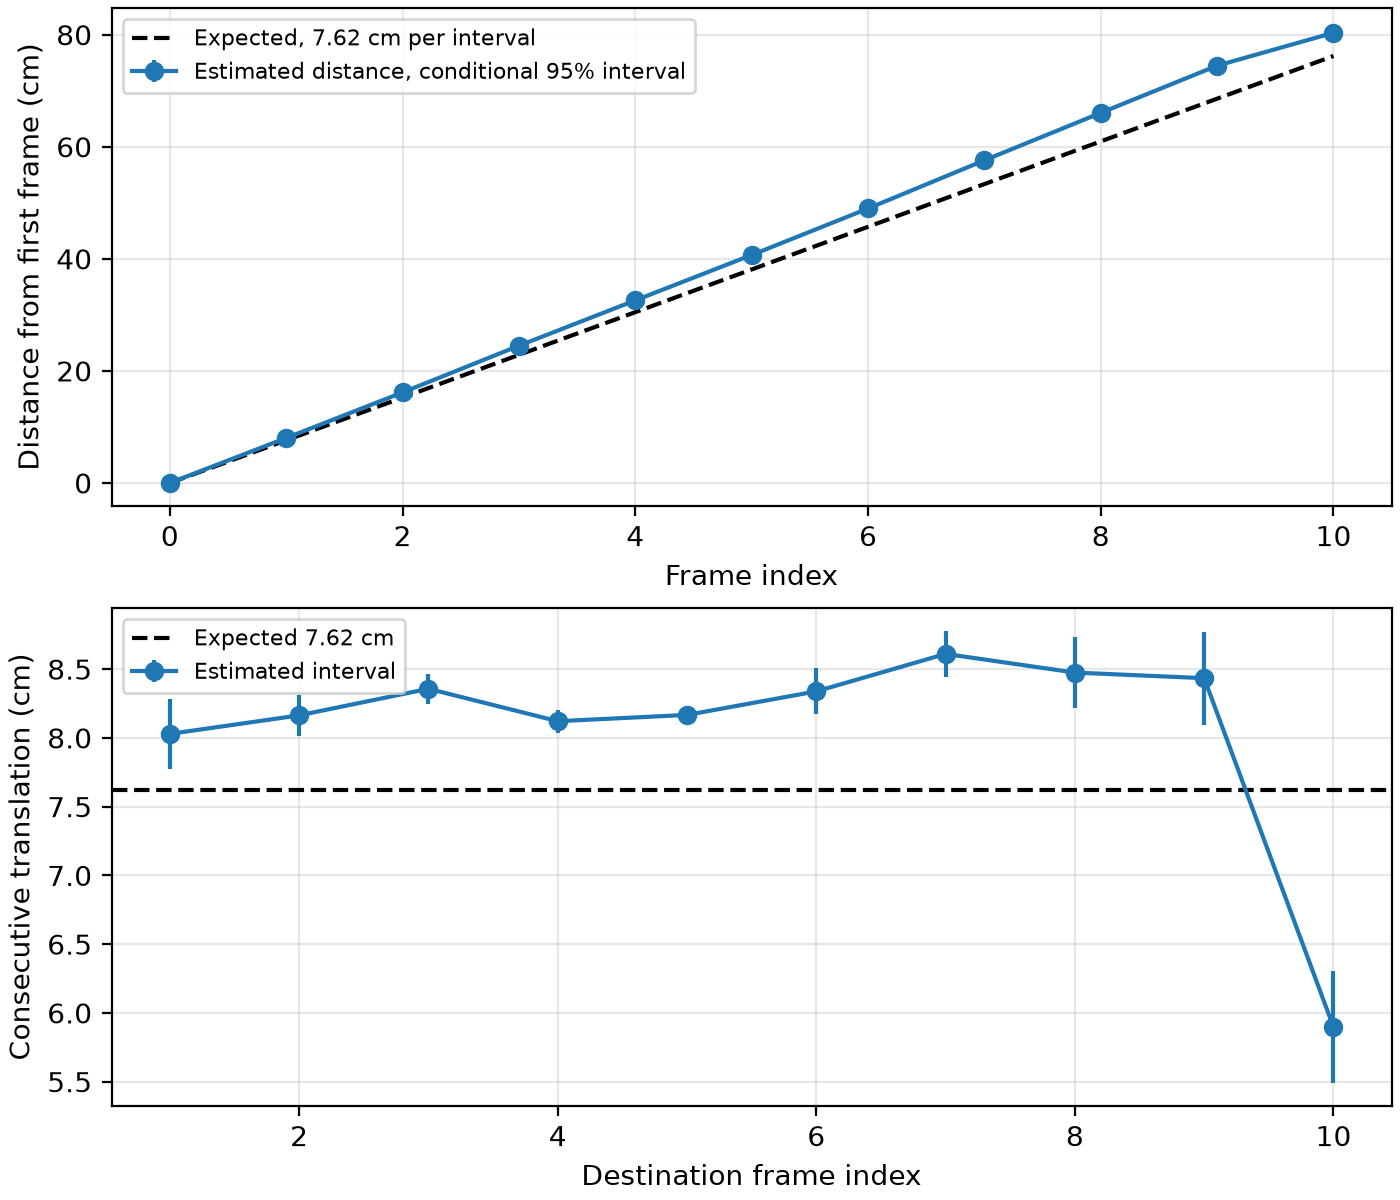
\includegraphics[width=\columnwidth]{motion_comparison.png}
\caption{Initial-frame displacement and consecutive translation compared with the measured spacing. Error bars are conditional 95\% intervals from the extra-credit analysis; they exclude systematic calibration, marker-size, and acquisition uncertainty.}\label{fig:comparison}
\end{figure}

These values support reasonable approximate motion over a 0.76 m span: estimated displacement grows consistently along the motion and has the correct order of magnitude, with a modest positive endpoint difference. They do not establish ruler-level accuracy. Intrinsic calibration, small marker-corner errors, physical marker-size tolerance, and deviations from an exactly fixed camera orientation can produce systematic differences. In particular, a low pixel residual alone cannot validate metric translation. No output is scaled to force agreement with the measured spacing.

\section{Task 5: Frame-by-Frame Evidence and Reproduction}
Table~\ref{tab:measurements} reports every input in timestamp order. X, Y, and Z are camera position components in the initial camera frame, not marker coordinates. ``Expected'' is nominal straight displacement from the first image, while ``Step'' is the norm between successive fitted positions. The first image defines zero displacement and has no preceding step.

\begin{table*}[t]\centering\caption{All measured camera positions and reference displacements, in centimeters. Time is the HHMMSS suffix of filenames dated 2026-11-24. The final column is the conditional 95\% half-width for $D_i$.}\label{tab:measurements}
\begin{tabular}{rr rrr rrrr}\toprule
Frame&Time&X&Y&Z&$D_i$&Expected&Step&$1.96\sigma_{D_i}$\\\midrule
\csname @@input\endcsname measurements.tex 
\bottomrule\end{tabular}
\end{table*}

For a repeat experiment, take the calibration views first using the same camera configuration, then the marked translation sequence described in Task 2. For the supplied sequence, run the following from the ME566 repository root:
\begin{lstlisting}[language=bash]
python3 -m venv .venv
.venv/bin/python -m pip install -r Homework/4/requirements.txt
.venv/bin/python Homework/4/calibrate_captures.py \
 Homework/4/hw4_captures/cal_caps \
 --output Homework/4/camera_cal.json
.venv/bin/python Homework/4/shared_orientation.py \
 Homework/4/hw4_captures/aruco_caps \
 --calibration Homework/4/camera_cal.json \
 --marker-length 0.10 --expected-step 0.0762 \
 --output Homework/4/outputs/captures_3inch_shared
.venv/bin/python Homework/4/build_report.py
.venv/bin/python -m unittest discover \
 -s Homework/4/tests -v
cd Homework/4/latex
pdflatex -interaction=nonstopmode -halt-on-error report.tex
pdflatex -interaction=nonstopmode -halt-on-error report.tex
\end{lstlisting}
The generated calibration records accepted source names, image dimensions, distortion, and per-view errors. The motion JSON records shared orientation, initial-relative transforms, positions, every interval, and whether spacing entered the fit (false). PNGs preserve full-resolution annotations; plots resize only for display. \code{build_report.py} regenerates numerical LaTeX fragments, figures, and the uncertainty JSON/covariance arrays. Python 3.12.3, OpenCV 5.0.0, and NumPy 2.5.4 were used. SciPy provides optimization and Matplotlib renders figures. Four regression tests pass, including synthetic exact/noisy shared-orientation recovery with unequal known translations.

\section{Task 6: Pose Uncertainty (Extra Credit)}
\subsection{Conditional covariance model}
Let $e(\theta)$ be the stacked 88 scalar pixel residuals from (\ref{eq:fit}), and let
\begin{equation}
J=\left.\frac{\partial e}{\partial\theta}\right|_{\widehat\theta},\qquad
\widehat\sigma^2=\frac{e^Te}{m-p}.
\end{equation}
Here $m=11(4)(2)=88$ and the numerical Jacobian rank is $p=36$, giving 52 residual degrees of freedom. OpenCV \code{projectPoints} returns derivatives with respect to rotation and translation. For each image, its first three columns fill the shared rotation block and its next three fill that image's translation block. The sign convention for predicted-minus-observed residuals matches those derivatives. With independent, zero-mean, equal-variance pixel errors and a locally linear projection, the parameter covariance is
\begin{equation}
\Sigma_\theta\approx\widehat\sigma^2(J^TJ)^{-1}.
\end{equation}
The fitted component-noise scale is $\SigmaPixel$ pixels. This differs from the 0.627-pixel two-dimensional corner RMS because one uses scalar residual degrees of freedom and the other averages squared 2D corner norms.

For a constant selection matrix $A_i$ implementing $p_i=t_0-t_i$, propagate
\begin{equation}
\Sigma_{p_i}=A_i\Sigma_\theta A_i^T.
\end{equation}
This retains cross-correlations between the initial and current translations and their shared rotation. For $D_i>0$,
\begin{equation}
g_i=p_i/D_i,\quad \sigma_{D_i}^2=g_i^T\Sigma_{p_i}g_i,\quad
D_i\pm1.96\sigma_{D_i}.
\end{equation}
The initial relative position is exactly zero by definition, so its relative covariance is zero. For each interval use a selector $B_i$ for $t_{i-1}-t_i$ and unit vector $h_i=(p_i-p_{i-1})/s_i$:
\begin{equation}
\sigma_{s_i}^2=h_i^TB_i\Sigma_\theta B_i^Th_i.
\end{equation}
Intervals are first-order Gaussian approximations, not a coverage guarantee.

\subsection{Measured uncertainty and interpretation}
At the final frame, one-standard-deviation component uncertainties are approximately $(0.166,0.127,0.812)$ cm in X, Y, and Z. Depth is less tightly constrained than the dominant image-plane motion. The endpoint distance has standard deviation 0.168 cm, giving $80.341\pm\EndpointCI$ cm at the approximate 95\% level. The standard deviations of the shared Rodrigues-vector components are approximately $(\SharedRxSD,\SharedRySD,\SharedRzSD)$ degrees; these are local parameter-component uncertainties, not Euler-angle uncertainties. Relative camera rotation remains fixed at zero; its zero variance is imposed rather than measured.

The 4.141 cm endpoint difference is much larger than this conditional random-noise interval. Therefore the covariance does not explain all disagreement with the measured spacing. It excludes uncertainty in $K,d$, printed size, guide spacing, focus changes, board flatness, correlated corner errors, and the constant-orientation assumption. It must not be reported as total physical pose accuracy. \code{uncertainty.json} and \code{pose_covariance.npz} include per-frame standard deviations, the full parameter covariance, relative-position covariances, and Jacobian for inspection.

\appendices
\section{OpenCV and Optimization Calls}
All dimensions passed to OpenCV are (width, height); pose coordinates are meters and radians. The five-coefficient model is used without fisheye or rational-model flags. Table~\ref{tab:calls} states the nontrivial calls and settings, including initialization used by the detector. Parameters not explicitly set use installed OpenCV defaults; dependency versions above identify the executed implementation.
\begin{table*}[t]\centering\scriptsize
\caption{Special functions, actual parameters, and their role}\label{tab:calls}
\begin{tabular}{L{.43\textwidth}L{.51\textwidth}}\toprule
Call / settings & Meaning\\\midrule
\code{imread(path,IMREAD_GRAYSCALE)}; \code{imread(path)}; \code{imwrite(path,image)} & Calibration decodes one intensity channel; pose/annotation uses BGR color. PNG writes use encoder defaults and their success is checked.\\
\code{findChessboardCornersSB(gray,(9,6),CALIB_CB_NORMALIZE_IMAGE)} & Find 54 inner corners; normalization enables histogram normalization before detection. Returned subpixel locations are used directly.\\
\code{calibrateCamera(objects,corners,(2992,2992),None,None)} & Joint intrinsic/distortion and per-board-pose fit with default flags 0, estimating $k_1,k_2,p_1,p_2,k_3$. No intrinsic guess. Default stopping criteria: 30 iterations and machine epsilon.\\
\code{getPredefinedDictionary(DICT_4X4_50)}; \code{generateImageMarker(dictionary,0,600,borderBits=1)} & Select marker dictionary; generate ID 0 at 600 square pixels with a one-cell black border for repeat printing. Printing must enforce the measured 10 cm outer square.\\
\code{DetectorParameters()}; \code{cornerRefinementMethod=CORNER_REFINE_SUBPIX} & Enable subpixel refinement. Executed defaults include maximum window 5 pixels, 30 iterations, minimum accuracy 0.1; adaptive threshold window min/max/step 3/23/10, constant 7, and one border bit.\\
\code{ArucoDetector(dictionary,params).detectMarkers(gray)}; \code{cvtColor(image,COLOR_BGR2GRAY)} & Detect ordered quadrilaterals and IDs from grayscale. Refined corners are full-resolution image coordinates.\\
\code{solvePnPGeneric(P,q,K,d,flags=SOLVEPNP_IPPE_SQUARE)} & Square-specific candidate poses in the stated corner order; detector initialization evaluates positive depth and pixel RMSE.\\
\code{solvePnP(P,q,K,d,flags=SOLVEPNP_ITERATIVE)} & Iterative PnP initialization without an extrinsic guess; final joint fit uses its per-frame translations and tries each initialized rotation.\\
\code{Rodrigues(r)}; \code{projectPoints(P,r,t,K,d)} & Convert rotation vector to matrix; project metric corners with distortion. Returned Jacobian supplies rotation/translation derivatives for uncertainty.\\
\code{drawDetectedMarkers(image,corners,ids)}; \code{drawFrameAxes(image,K,d,r,t,0.05,2)} & Draw green outlines/IDs and RGB XYZ axes of length 5 cm and thickness 2 pixels.\\
\code{putText(image,text,position,FONT_HERSHEY_SIMPLEX,.5,color,thickness)} & Status labels begin at $(10,24)$ and advance 24 pixels; black thickness 3 under white thickness 1 improves visibility.\\
\code{drawChessboardCorners(image,(9,6),corners,found)}; \code{cvtColor(image,COLOR_BGR2RGB)} & Calibration overlay and correct report colors; no change to fitted coordinates.\\
\code{least_squares(residual,x,method='lm',max_nfev=3000,ftol=1e-11,xtol=1e-11,gtol=1e-11)} & SciPy joint nonlinear least squares, linear loss and default two-point numerical derivatives for optimization. OpenCV analytic projection derivatives are used separately for covariance.\\\bottomrule
\end{tabular}
\end{table*}

\section{Source Code and Submission Contents}
The accompanying \code{outputs/hw4_source.zip} contains the report source, generated numerical tables and figures, camera calibration, dependency list, tests, and Python modules. The executable shared-orientation method appears in \code{shared_orientation.py}; \code{build_report.py} includes the complete uncertainty calculation. The independent-pose CLI \code{main.py} is also included, but the reported experiment uses the shared-orientation command above. The supplied \code{io/image_reader.py} remains unchanged. Submit the original capture archive \code{hw4_captures.zip} with this source package and PDF so that another student can reproduce the measurements. Generated full-resolution annotations and JSON are in \code{outputs/captures_3inch_shared/}.

\begin{table}[ht]\centering\small\caption{Source file roles}
\begin{tabular}{L{.42\columnwidth}L{.48\columnwidth}}\toprule
File & Purpose\\\midrule
\code{calibrate_captures.py} & Checkerboard detection and intrinsic calibration.\\
\code{aruco/calibration.py} & Load/validate camera matrix and distortion.\\
\code{aruco/detection.py} & Marker detection, corner refinement, initial pose checks.\\
\code{shared_orientation.py} & Shared rotation/per-image translation fit and annotation export.\\
\code{aruco/visualization.py} & Marker outlines, frame axes, position labels.\\
\code{aruco/motion.py}, \code{main.py} & General rigid-transform pipeline and CLI.\\
\code{build_report.py} & Measured tables, figures, Jacobian covariance.\\
\code{tests/} & Synthetic geometry and CLI regression tests.\\
\code{camera_cal.json}, \code{requirements.txt} & Fitted intrinsics and dependencies.\\\bottomrule
\end{tabular}\end{table}
\begin{thebibliography}{2}
\bibitem{aruco} OpenCV, ``Detection of ArUco Markers.'' [Online]. Available: \url{https://docs.opencv.org/4.x/d5/dae/tutorial_aruco_detection.html}.
\bibitem{calib} OpenCV, ``Camera Calibration and 3D Reconstruction.'' [Online]. Available: \url{https://docs.opencv.org/4.x/d9/d0c/group__calib3d.html}.
\end{thebibliography}
\end{document}
